\section{Analysis} \label{sec:analysis}

We provide a brief quantitative analysis of the scale and efficacy of Tutela heuristics.
\begin{figure}[h!]
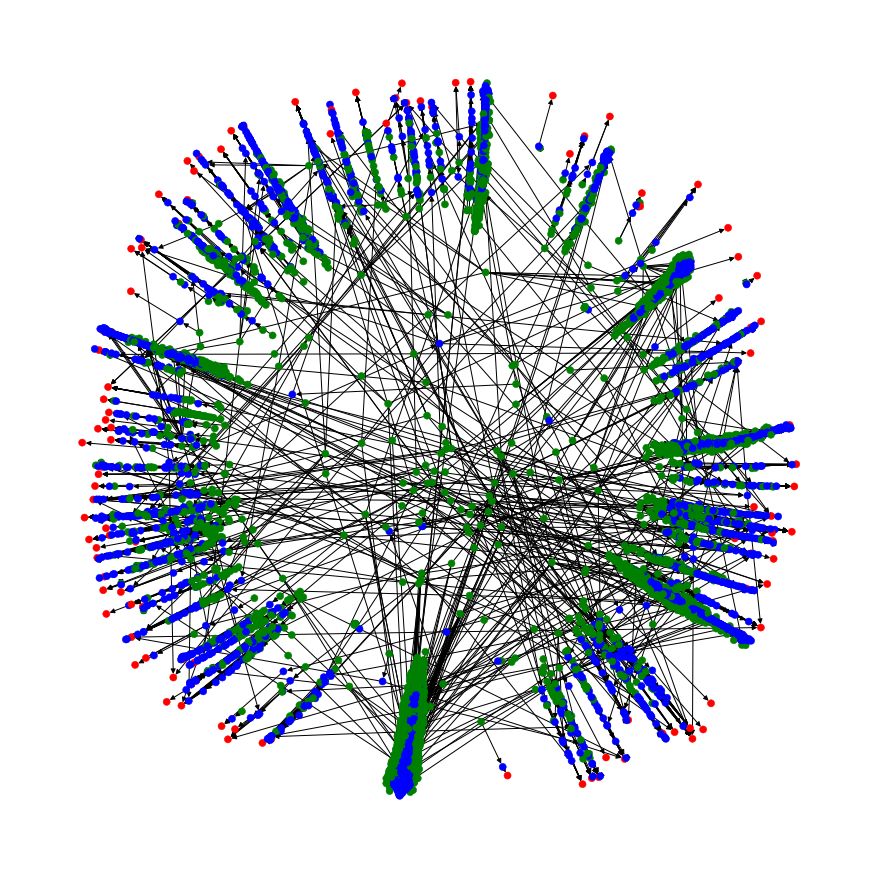
\includegraphics[width=\linewidth]{figures/dar_graph.png}
\caption{10k subgraph of 26M graph created via deposit address reuse. Contains EOA (green), deposits (blue), and exchanges (red).}
\label{fig:dargraph}
\end{figure}
\subsection{Ethereum Heuristics}

Using DAR, we found 26M EOA addresses, resulting in 2.5M clusters of Ethereum addresses. The average cluster size contains 4.3 ($\pm$ 8.6) EOA addresses; the largest cluster contains 2.1k EOA addresses. Figure~\ref{fig:dargraph} shows a visualization of 10,000 random nodes from the DAR graph. In particular, we observe interesting structure with many small clusters scattered uniformly, balanced by several large clusters in the perimeter.

Next, we can measure the quality of the DAR clusters using a held out ``test set'' of known clustered addresses. We obtain such a set from \cite{beres2021blockchain} where 1,028 clusters of addresses (average size of 4.0 $\pm$ 3.6 EOA addresses per cluster) are derived from ENS names. We find a recall of 39.4\% using Tutela heuristics. While there is room for improvement, we are cautiously optimistic that DAR was able to recover a nontrivial number without any knowledge of ENS names. This provides evidence for the generality of DAR clusters.

\begin{figure}[h!]
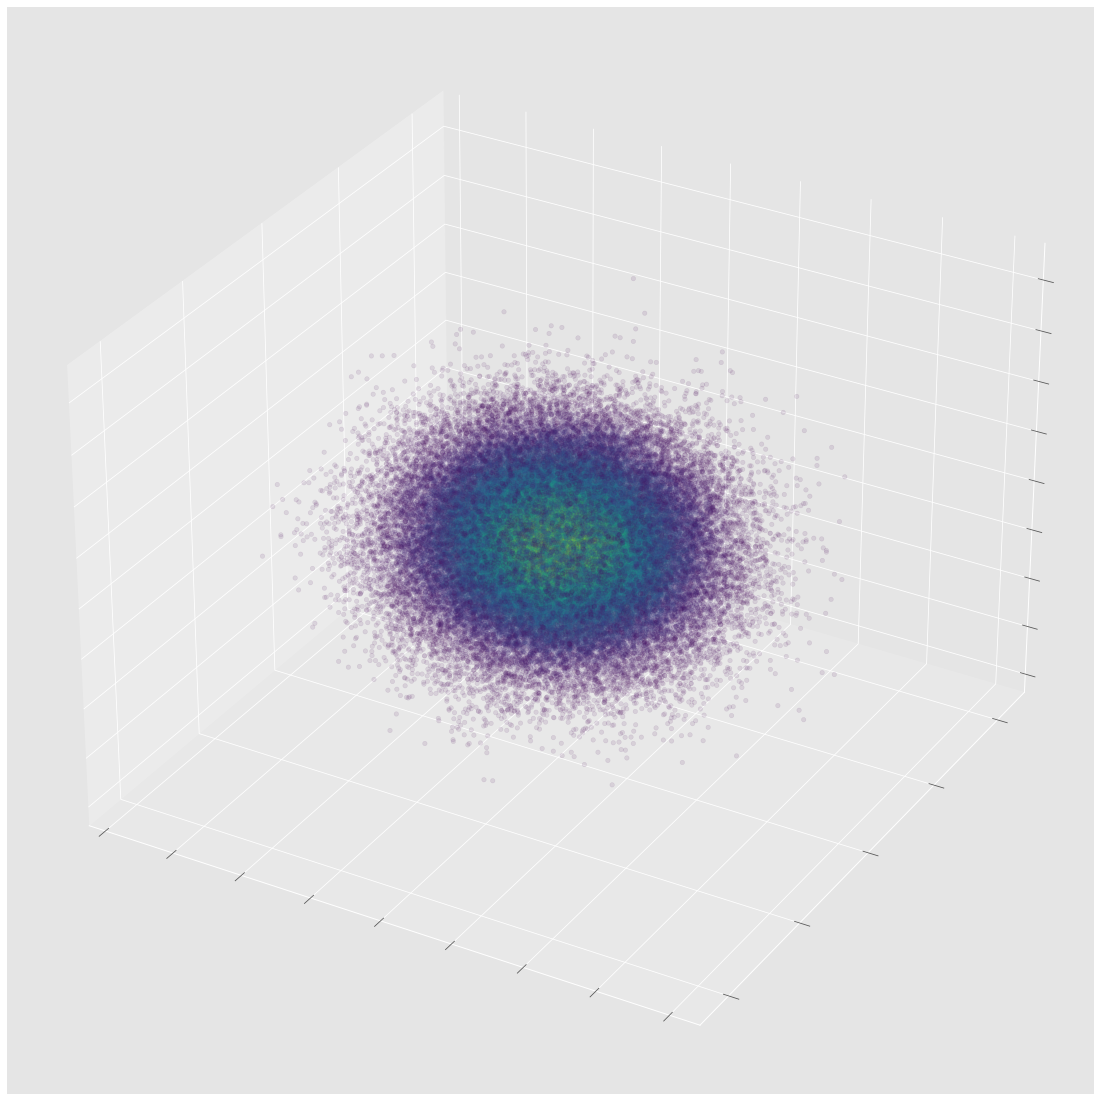
\includegraphics[width=\linewidth]{figures/diff2vec_sample}
\caption{100k random subset of 131M embedding of Ethereum addresses projected from to 3D using PCA.}
\label{fig:diff2vecgraph}
\end{figure}
Using Node, we found 131M clusters of Ethereum addresses, with each cluster having exactly 9 members by design (10 including itself). Figure~\ref{fig:diff2vecgraph} shows a visualization of 100,000 random embeddings of Ethereum addresses from the NODE set, where embeddings are projected down to two dimensions using PCA (trained on a subset of 1M address embeddings). The color in Figure~\ref{fig:diff2vecgraph} shows the density, estimated using a Gaussian kernel, where a lighter (yellow) color represents higher density. That is, the figure shows a non-hollow ball of address embeddings. For any query address, Tutela returns the closest neighbors from the point cloud. 
More analysis on NODE embedding quality will be conducted in future work.

\subsection{Tornado Cash Heuristics}

Of the 97.3k Tornado Cash equal user deposits, we found 42.8k are potentially compromised: 18.6K from the address match reveal, 102 from the unique gas price reveal, 18.9K from the linked ETH reveal, 16.2K from the multi-denomination reveal, and 358 from the TORN mining reveal (with overlap between reveals). Splitting this by pool, we find the anonymity set to be reduced by 42\% ($\pm$ 14\%) on average. Figure~\ref{fig:tcashgraph} shows the uncompromised anonymity sets by pool.

We find that some of the pools could be heavily compromised (such as the cDAI and WBTC pools), whereas other pools are less effected (e.g. USDC). In summary, while many of the Tornado Cash heuristics are simple, they are quite powerful. These findings could help Tornado Cash developers and users alike, measure and understand the degree of protection to user privacy.

\begin{figure}[h!]
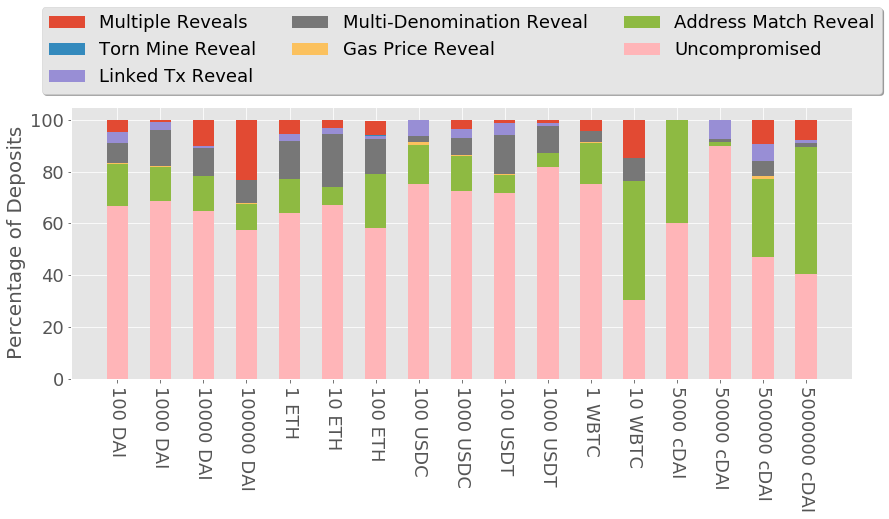
\includegraphics[width=\linewidth]{figures/tornado_graph.png}
\caption{Plot of the percentage of compromised versus uncompromised (purple) deposits by pool. }
\label{fig:tcashgraph}
\end{figure}